\chapter{Momentum and Energy Transfer in Packed Beds}\label{sec:survey-packed-beds}
We review the momentum and exchange between a fluid moving through a porous medium and the drag force correlations that are used in engineering practice. Then we walk through the many modes of energy exchange between contacting particles and particles with an interstitial gas.
%%%%%%%%%%%%%%%%%%%%%%%%%%%%%%%%%%%%%%%%%%
\section{Pressure Drop Across Packed Beds} \label{sec:modeling-pressure-drop}
%%%%%%%%%%%%%%%%%%%%%%%%%%%%%%%%%%%%%%%%%%
% Hill, Kock, \& Ladd\cite{Hill2001a}

% small Reynolds numbers

% simple cubic, face-centered cubic, random arrays

% drag force phi --> close-packed limits

% for small solid volume fraction, simulation similar to theory, therefore first inertial contribution to the drag force, when scaled with the Stokes drag force on a single sphere in open fluid, is proportional to the square of the Re #. Scaling persists --> close-packed limits.

% Inertial contribution to the drag force decreases with increasing solid volume fraction.

% Unsteady force is dominated by quasi-steady drag and added-mass forces.
%%%%%%%%%%%%%%%%%%%%%%%%%%%%%%%%%%%%%%%%%%
%\input{}
%%%%%%%%%%%%%%%%%%%%%%%%%%%%%%%%%%%%%%%%%%
\subsection{Kozeny-Carman Correlation for Pressure Drop}
P.C. Carman\cite{Carman1997}, using Kozeny's Equation as a starting point, derived a formula for the average velocity of a laminar flow through a randomly packed beds at the close-packed limit,

\begin{equation}\label{eq:K-C-velocity}
	U = \left(\frac{L}{L_e}\right)^2\frac{\epsilon^3}{k_0\mu S^2}\frac{\Delta p}{L}
\end{equation}

where $\mu$ is the viscosity, Carman called the tortuosity ($L_e/L$) the ratio of the actual path of a streamline through the pore space, $L_e$, to the length of packing, $L$. $S$ is the particle surface area per unit volume of the bed. For a bed of spheres this is $S = 6(1-\epsilon)/d_p$. The fluid void fraction, $\epsilon$ is obviously the complement to the packing fraction $\epsilon = 1 - \phi$ that we have used throughout this work. The constant, $k$, varies between materials and packings but for regular spheres is found experimentally to be $k\approx 5.0$. $\Delta p/L$ is the pressure drop per unit length of flow in the packed bed.

We rearrange Eq.~\ref{eq:K-C-velocity} as

\begin{equation}\label{eq:K-C-pressure}
	\frac{\Delta p}{L} = \frac{180 U \mu}{d_p^2} \frac{(1-\epsilon)^2}{\epsilon^3}
\end{equation}

The pressure gradient acting upon the fluid in the packed bed must be balanced by the drag force of all the particles in the bed. If we assume some average force, $\langle f \rangle$, as the ensemble average of the particle drag forces, we can write

\begin{equation}
	\frac{\Delta p}{L} = n \langle f \rangle
\end{equation}

where $n$ is the number density of particles in the bed. We relate the number density in terms of the packing fraction as

\begin{equation}
	n = \frac{6\phi}{\pi d_p^3} = \frac{6(1-\epsilon)}{\pi d_p^3}
\end{equation}

Thus the average drag per particle in this flow is

\begin{equation}\label{eq:average-drag}
	\langle f \rangle = \frac{\Delta p}{L}\frac{\pi d_p^3}{6(1-\epsilon)}
\end{equation}

We will nondimensionalize the average drag force based on the classic Stokes force, drag force of a single particle in unbounded fluid,

\begin{equation}\label{eq:non-dim-drag}
	F = \frac{\langle f \rangle}{3\pi \mu d_p U}
\end{equation}

and when we plug in Eq.~\ref{eq:average-drag} to Eq.~\ref{eq:non-dim-drag} we have

\begin{equation}
	F_{kc} = \frac{\Delta p}{L}\frac{\pi d_p^3}{6(1-\epsilon)}\frac{1}{3\pi \mu d_p U}
\end{equation}

which, with the substitution of the Kozeny-Carman pressure (Eq.~\ref{eq:K-C-pressure}), becomes

\begin{equation}
	F_{kc} = \frac{180 U \mu}{d_p^2} \frac{(1-\epsilon)^2}{\epsilon^3}\frac{\pi d_p^3}{6(1-\epsilon)}\frac{1}{3\pi \mu d_p U}
\end{equation}

or simply

\begin{equation}\label{eq:K-C-non-dim}
	F_{kc} = 10\, \frac{1-\epsilon}{\epsilon^3}
\end{equation}

Carman points out\cite{Carman1956} the limitations of the Kozeny-Carman equation. Built into the equation is the assumption that the range of pore size and shape is fairly isotropic and similarly the tortuosity through the packed bed is relatively uniform. In the form we have used with Eq.~\ref{eq:K-C-non-dim}, we have also assumed spherical particles in random packing near the close-packed limit ($\phi \rightarrow 0.64$) with laminar flow at low Reynolds numbers. Carman provided modifications to cases of extremely high porosity and non-spherical, non-regular packings in his book from 1956.\cite{Carman1956}

\subsection{Ergun Correlation for Pressure Drop}

Another correlation that is perhaps more commonly used in general is the Ergun equation.\cite{ergun1952fluid} Ergun's correlation is an empirical fit to a vast amount of experimental data. His pressure drop per length is 

\begin{equation}\label{eq:ergun-pressure}
	\frac{\Delta p}{L} = \frac{150 U \mu}{d_p^2} \frac{(1-\epsilon)^2}{\epsilon^3} + \frac{1.75 \rho U^2}{d_p}\frac{1-\epsilon}{\epsilon^3}
\end{equation}

We nondimensionalize the Ergun equation of Eq.~\ref{eq:ergun-pressure} in the same form as Eq.~\ref{eq:K-C-non-dim} to find

\begin{equation}\label{eq:ergun-non-dim}
	F_e = 8.33 \, \frac{1-\epsilon}{\epsilon^3} + 0.18 \, \frac{\Re}{\epsilon^3}
\end{equation}

where we see the Reynolds number dependence in the second term on the right side of Eq.~\ref{eq:ergun-non-dim}. Comparing this to the nondimensionalized drag force of the Kozeny-Carman relation (Eq.~\ref{eq:K-C-non-dim}), we see that the first term on the right hand side is essentially the same but Ergun's equation underpredicts Stokes flow by roughly 20\% (8.33 to 10.0). This is understandable as Ergun's equation was meant to fit a wide range of flow (finite-to-large $\Re$), including turbulent flow, whereas the Kozeny-Carman was meant specifically to apply to Stokes flow-type laminar packed beds.

\subsection{Koch-Hill-Lad Correlation for Pressure Drop}
Koch, Hill, \& Ladd studied packed bed flow with high-precision lattice-Boltzmann simulations to develop correlations for drag in a packed bed over a wide range of packing fractions and Reynolds numbers.\cite{Koch2001,Hill2001a,Hill2001} They studied ordered arrays of spheres at various flow angles with dilute arrays (interstitial Reynolds number greater than particle Reynolds number), up to dense ordered arrays, and random arrays.

They consider the drag force as a sum of viscous and inertial stresses. Based on scaling arguments, the viscous and inertial contributions to $F$ are expected to be independent of $\Re$ and linearly proportional to $\Re$, respectively (in much the same form as Ergun's empirical fit of Eq.~\ref{eq:ergun-non-dim}). Thus their numerical results were fit to the form

\begin{equation}\label{eq:khl-correlation-appendix}
	F = F_0(\phi) + F_3(\phi)\Re
\end{equation}

where 

\begin{equation}
F_0 = \begin{cases}
	\frac{1+3(\phi/2)^{1/2} + (135/64)\phi\ln\phi + 16.14\phi}{1 + 0.681\phi - 8.48 \phi^2 + 8.16\phi^3} & \text{if $\phi < 0.4$}\\
	10.0\,\frac{\phi}{(1-\phi)^3} & \text{if $\phi > 0.4$} 
	\end{cases}
\end{equation}

and

\begin{equation}
	F_3 = 0.0673 + 0.212\phi + 0.0232 \frac{1}{(1-\phi)^5}
\end{equation}

Koch, Hill, \& Ladd\cite{Hill2001, Koch2001, Gruber2012, Benyahia2006} compare their results with data from experiments. They found that at smaller Reynolds number and larger solid volume fractions, the rate of increase of drag force increases with the Reynolds number in much the same way predicted by Ergun’s equation. However, at solid volume fractions smaller than those that can be achieved in physical experiments, at the largest Reynolds numbers, the rate of drag force increase is significantly smaller than the value predicted by Ergun's equation.

For Stokes-flow (and near-Stokes-flow), the drag force computed from their lattice-Boltzmann simulations were indistinguishable from experimental data over all ranges of packing fractions achievable in controlled experiments. The correlation fit to their data for small Reynolds number and large packing fraction is simply the Kozeny-Carman relationship -- which was itself generated with coefficients matching experimental data so it is no surprise their correlation fits that phase space of $\phi-\Re$.

\subsection{Correlation Comparisons}
We have given three correlations relating a nondimensional drag force to packing fraction and Reynolds number. The first, the Kozeny-Carman equation, is applicable at small Reynolds number and broad range of packing fraction. The second, the Ergun equation, is applicable at a broad range of Reynolds number but is most accurate at higher packing fractions and also under-predicts drag at low Reynolds numbers. Finally, the third correlation by Koch, Hill, \& Ladd (KHL), extended the drag correlations over a much more broad packing fraction and Reynolds numbers than is possible with physical experiments. 

Here we simply provide a graphical comparison of the relationships that demonstrates when the classic correlations of Kozeny-Carman and Ergun match the correlation of KHL and when they diverge.
\begin{figure}[!ht]
	\centering
	\begin{subfigure}[b]{0.45\textwidth}
		\centering
		\includegraphics[width=\textwidth]{figures/pressure-drop-correlations/Re0.png}
	\end{subfigure}
	\begin{subfigure}[b]{0.45\textwidth}
		\centering
		\includegraphics[width=\textwidth]{figures/pressure-drop-correlations/Re10.png}
	\end{subfigure}
	
	\begin{subfigure}[b]{0.45\textwidth}
		\centering
		\includegraphics[width=\textwidth]{figures/pressure-drop-correlations/Re20.png}
	\end{subfigure}
	\begin{subfigure}[b]{0.45\textwidth}
		\centering
		\includegraphics[width=\textwidth]{figures/pressure-drop-correlations/Re30.png}
	\end{subfigure}

	\begin{subfigure}[b]{0.45\textwidth}
		\centering
		\includegraphics[width=\textwidth]{figures/pressure-drop-correlations/Re40.png}
	\end{subfigure}
	\begin{subfigure}[b]{0.45\textwidth}
		\centering
		\includegraphics[width=\textwidth]{figures/pressure-drop-correlations/Re50.png}
	\end{subfigure}
	\caption{Comparison of pressure drop correlations over a range of packing fractions and Reynolds numbers.}
\label{fig:p-drop-correlations}
\end{figure}

Later, in \cref{sec:modeling-cfd-dem}, we will return to these correlations as we discuss the computational groundwork of the CFD-DEM coupling routine.



\FloatBarrier




%%%%%%%%%%%%%%%%%%%%%%%%%%%%%%%%%%%%%%%%%%
\section{Heat Transport in Packed Beds} \label{sec:modeling-heat-transfer}
%%%%%%%%%%%%%%%%%%%%%%%%%%%%%%%%%%%%%%%%%%
In our analysis of the momentum of packed beds, we focused entirely on the exchange of momentum between a fluid passing through a packed bed. The mechanics of contacting particles will be dealt with entirely within the framework of the discrete element method, to be discussed in \cref{sec:modeling-dem}. But now as we move to analyze the heat transfer in a packed bed, we will consider both inter-particle modes of heat transfer as well as particle-fluid convection. 


\begin{figure}[t]
	\centering
	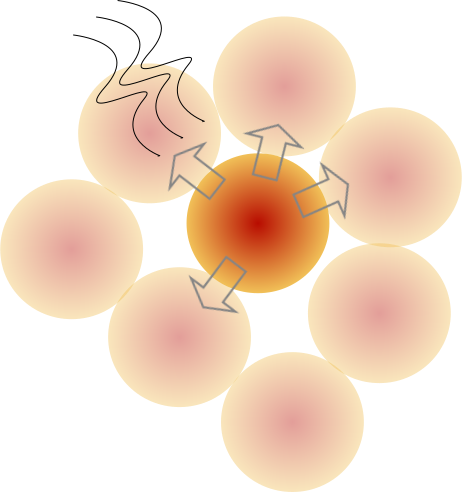
\includegraphics[width=0.35\textwidth]{figures/pebble-complete-heat-transfer}
	\caption{An illustration highlighting a single particle transferring energy into a passing fluid and neighboring particles in the ensemble.}\label{fig:peb-comp-ht}
\end{figure}

Looking at the particle highlighted in Fig.~\ref{fig:peb-comp-ht}, we see many pathways for heat to be transferred inside the ensemble. The most significant are:

\begin{enumerate}
\item Conduction through the contact area between contacting particles.
\item Conduction through the stagnant fluid between near, non-contacting particles.
\item Conduction through the stagnant fluid between contacting particles.
\item Advection of energy by the fluid to contacting- and downstream particles.
\item Radiation between the surfaces of contacting particles.
\item Radiation between particles of adjacent voids.
\item Heat generation internally in the particle.
\end{enumerate}

We will address the inter-particle conduction in \cref{sec:ht-pebble-conduction} wherein we derive a formula for heat conductance between contacting, elastic spheres. The complex interaction of energy in a particle with a fluid (conduction through film regions, convection with passing fluid, etc.) will all be dealt with using correlations for packed beds; this is done in \cref{sec:particle-convection}. We will briefly discuss some literature where researchers have dealt with the radiation between particles in a packed bed but do not include the terms in our current models. Finally, the last mode of heat transfer is trivially accounted for with a heat source term,

\begin{equation}\label{eq:nuclear-heating-term}
	Q_g = q'''V
\end{equation}

where $q'''$ is a known volumetric heating rate and $V$ is the volume of our particle. In practice, we will know a volumetric heating rate from the location and geometry of the solid breeder volume. The volume of the sphere is $V = \frac{\pi}{6} d_p^3$.

In the following sections we will expand upon the details of the modes of heat transfer considered for our packed beds. They forms of equations used will be written in a way as to be easily implemented directly into the DEM computational framework, to be discussed later in \cref{sec:modeling-dem}.

% The transient energy balance for an irradiated pebble, shown in Fig.~\ref{fig:peb-comp-ht}, in a packed bed with flowing interstitial gas is given by Eq.~\ref{eq:single-pebble-energy},

% \begin{equation}\label{eq:single-pebble-energy}
% 	\rho V C \frac{\mathrm{d}T}{\mathrm{d}t} = \dot{Q}_g + \dot{Q}_\text{conduction} + \dot{Q}_\text{convection} + \dot{Q}_\text{radiation}
% \end{equation}



%%%%%%%%%%%%%%%%%%%%%%%%%%%%%%%%%%%%%%%%%%
\subsection{Inter-particle Heat Conduction}\label{sec:ht-pebble-conduction}

When two particles come into contact, energy is transmitted through their region of contact. For this discussion, we assume the particles are spherical, elastic, in vacuum, and we neglect radiation transfer between them. If the two particles are at temperatures $T_i$ and $T_j$ we can quantify the amount of energy transferred between them with a commonly used practice of a contact conductance, $H_c$:
\begin{equation}\label{eq:pebble-conduction-heat-transfer}
	Q_{ij} = H_{c}(T_i - T_j)
\end{equation}

The subscripts are omitted for clarity, but obviously there is a unique $H_c$ per pair of contacting particles. We note that the heat conductance, unlike standard heat transfer coefficients, has units of \si{\watt\per\kelvin}.

Batchelor and O'Brien\cite{Batchelor1977} developed a formulation of similar form and then made the brilliant observation that the temperature fields in the near-region of contacting spheres are analogous to the velocity potential of an incompressible, irrotational fluid passing from from one reservoir to another through a circular hole in a planar wall separating the two reservoirs. With the analogy, they could make use of the fluid flow solution to write the total flux across the circle of contact just as Eq.~\ref{eq:pebble-conduction-heat-transfer} with the heat conductance as

\begin{equation}\label{eq:batchelor-pebble-conductance}
	H_c = 2k_ra
\end{equation}

where $k_r$ is the conductivity of the contacting solids and $a$ is the radius of contact. In \cref{sec:hertz-theory}, with Hertz theory we found the contact radius in terms of the contact pressure. Here, we give the radius in terms of the compression force acting on the bodies,

\begin{equation}
	a =  \left(\frac{3}{4}\frac{R^*}{E^*}\right)^{1/3}F_n^{1/3}	
\end{equation}

as before, $\frac{1}{E^*} = \frac{1-\nu_1^2}{E_1} + \frac{1-\nu_2^2}{E_2}$ and $\frac{1}{R^*} = \frac{1}{R_1} + \frac{1}{R_2}$. 

In the development of Eq.~\ref{eq:batchelor-pebble-conductance}, Batchelor and O'Brien had assumed the two contacting spheres to be of equal conductivity, $k_r$. Cheng\etal\cite{Cheng19994199} proposed a slightly modified conductance which allows for contacting materials of different thermal conductivity. They have,

\begin{equation}\label{eq:cheng-modification-batchelor}
	H_c = 2k^*a = 2k^* \left(\frac{3}{4}\frac{R^*}{E^*}\right)^{1/3}F_n^{1/3}
\end{equation}

where $\frac{1}{k^*} = \frac{1}{k_i} + \frac{1}{k_j}$. As well as being a more general, flexible formulation, the models analyzed by Cheng\etal\cite{Cheng19994199} are in good agreement with experiments. In the DEM numerical structure, we use the form given by Eq.~\ref{eq:cheng-modification-batchelor}.

Furthermore, Batchelor and O'Brien developed Eq.~\ref{eq:batchelor-pebble-conductance} with the assumption of two contacting particles in vacuum but, once developed, showed\cite{Batchelor1977} that this form is still valid when immersed in a fluid providing that the thermal conductivity ratio of solid and fluid is well above unity. The condition is expressed as,

\begin{equation}\label{eq:conductance-validity-fluid}
	\frac{ k_r }{ k_f } \frac{a}{R^*} \gg 1
\end{equation}

The term $\frac{a}{R^*}$, from \cref{sec:hertz-theory}, is necessarily much less than 1 for Hertz theory to be applicable. Thus for fluid in vacuum, the condition is identically satisfied but we must consider inaccuracies if we introduce an interstitial fluid with low conductivity ratios; for lithium ceramics in helium, the ratio is approximately $\frac{k_r}{k_f} \approx 10$.

As we step back from the contact of a single pair of particles and consider a particle in an ensemble with many contacts, we must again consider the validity of applying Eq.~\ref{eq:cheng-modification-batchelor} at each contact. Vargas and McCarthy\cite{Vargas2002a}, proposed introducing a conduction Biot number to relate resistance to heat transfer internal to the particle with the resistance between particles. We use the following form

\begin{equation}
	\Bi_c = \frac{H_c}{k^* d_p} = 2\frac{a}{d_p}
\end{equation}

Then if $\Bi_c \ll 1$, the individual energy transferred between each point of contact can be decoupled. The Biot number criteria is already satisfied for Hertz theory to be valid; having assumed that $\frac{a}{d_p} \ll 1$. Therefore the total heat transferred out of a single particle with $Z$ contacts is the summed contribution of individual contacts, 

\begin{equation}
	Q_i = \sum_j^Z Q_{ij}
\end{equation}

The contact conductance we use, Eq.~\ref{eq:cheng-modification-batchelor}, which is built upon the solution of Batchelor and O'Brien\cite{Batchelor1977}, has been implemented by others in a variety of studies\cite{Vargas2001, Chaudhuri2006, Zhou2009,Cheng19994199}. However, in many other fields, the researchers are interested in such things as the parallel conduction through a stagnant interstitial gas\cite{Bu2013} or the temporary conduction during impact of fluidized beds\cite{Zhu2008,Zhang2011,Wu2011,Li2000}. In such cases, the formula for conductance can be quite different but are not appropriate for the physics of our packed beds.

% Nevertheless, for the packed beds of ceramic spheres for which we are working towards modeling, the heat conductance of Eq.~\ref{eq:cheng-modification-batchelor} is an appropriate and valid form. The interstitial gas, be it stagnant or moving, will be incorporated the influence of an interstitial gas, it will be done in such a way as to leave the DEM heat transfer intact and only add an energy source term to stand in for the interaction with the fluid. The details will be discussed in \cref{sec:cfdem-heat-transfer}, but for now we conclude with a solid conduction theory that will be implemented in the discrete element method computations.


\subsection{Nusselt Number for Spheres in Packed Beds}\label{sec:particle-convection}

Historically, in the treatment of packed beds for heat transfer, engineers developed relationships between overall heat transfer coefficients to the log-mean temperature of the bed. The Nusselt number correlation was applicable to the bed overall rather than any discrete particle inside of the bed. The correlations will be useful for validating our models of helium flow through packed beds of lithium ceramics.


Recently, however, experimental and numerical research has focused on the heat transfer at the scale of a particle as a component of dilute or dense packed beds. These correlations will be useful for applying to single discrete elements in our DEM framework.

\begin{equation}
	Q_\text{convection} = -hA_r(T_r-T_f)
\end{equation}

where $T_r$ is the temperature of the solid with surface area, $A_r$, and $T_f$ is the local bulk temperature of the passing fluid.

%~~~~~~~~~~~~~~~~~~~~~~~~~~~~~~~~~~~~~~~~~~~~~~~~~~~~~~~~~~~~~~~~~~~~~~~~
\subsubsection{Van Lew }

In their analysis of solar thermal storage devices, Van Lew\etal~derived a form of heat transfer coefficient based on the Chilton-Colburn analogy.\cite{vanlew133} The form of their solution followed from the form used by Nellis and Klein \cite{Nellis2009} in heat exchangers. The heat transfer coefficient used by Van Lew\etal~reads
% To determine the coefficient, the details of geometry are required.  Necessary values are the porosity, or void fraction, $\epsilon$, and the cross-sectional surface area of the storage tank, $A_t$.

% The heat transfer coefficient correlation is offered in terms of the Colburn $j_h$ factor.
% \begin{equation}
% j_h=\frac{\bar{h}}{G c_f} Pr_f^{2/3}
% \end{equation}
% The mass flux, G, is evaluated in terms of the specific surface area and mass flow rate:
% \begin{equation}
% G=\frac{\dot{m}}{\epsilon A_t}
% \end{equation}
% where $c_f$ is the specific heat capacity of the fluid and $Pr_f$ the Prandtl number of the fluid.  A correlation between $j_h$ and Reynolds number is found.  For a packed bed of spheres a modified Reynolds number has been suggested by Kays and London (1984) and is defined as:
% \begin{equation}
% Re=\frac{4 G r_{char}}{\mu_f}
% \end{equation}
% where $\mu_f$ is the viscosity of the fluid.  The characteristic radius $r_{char}$ is given as:

% where $d_p$ is the average diameter of the packed bed particle.

% The relationship between Colburn $j_h$ factor and Reynolds number was provided in Nellis and Klein.  The data was replotted and an interpolation yielded a functional relationship as:
% \begin{equation}
% jh=0.191 Re^{-.278}
% \end{equation}
% Therefore, the heat transfer coefficient is found through rearranging the above relationships, providing Eqn.~\ref{eq:h}:

\begin{equation}\label{eq:vanlew-htc}
	\Nu =0.191 N_v Re_G^{-.278} Pr_f^{-2/3}
\end{equation}
where the dimensionless grouping $N_v = \frac{\dot{m}D_hc_f}{\epsilon A_tk_f}$ and they used a modified Reynolds number based on the mass flux and hydraulic diameter of their storage tank,
\begin{equation}
	Re_G=\frac{4 \dot{m} r_{char}}{\epsilon \pi R_t^2\mu_f}
\end{equation}
where $R_t$ is the radius of the storage tank and with $r_char$ a characteristic radius (or hydraulic radius) of their packing, 
\begin{equation}
	r_{char}=\frac{\epsilon d_p}{4(1-\epsilon)}
\end{equation}
and $d_p$ is the nominal diameter of filler material.

While the simulations of thermoclines run by Van Lew\etal~predicted well the results of their experimental data\cite{vanlew133,Valmiki2012a} their correlation for heat transfer coefficient does not match theory as $\Re \rightarrow 0$. In a stationary fluid, $Nu = 2$ but in the correlation of Eq.~\ref{eq:vanlew-htc}, as $\Re \rightarrow 0$, $\Nu \rightarrow0$ and thus is not appropriate for the low-Reynolds flows inside the solid breeder volume.

%~~~~~~~~~~~~~~~~~~~~~~~~~~~~~~~~~~~~~~~~~~~~~~~~~~~~~~~~~~~~~~~~~~~~~~~~





%~~~~~~~~~~~~~~~~~~~~~~~~~~~~~~~~~~~~~~~~~~~~~~~~~~~~~~~~~~~~~~~~~~~~~~~~
% \subsubsection{Packed beds correlation: Whitaker}

% Definition of Reynolds number

% \begin{equation}
% 	\Re = \frac{D_p G}{\mu_b(1-\epsilon)}
% \end{equation}

% Definition of Nusselt number

% \begin{equation}
% 	\Nu = \frac{hD_p}{k_f}\frac{\epsilon}{1-\epsilon}
% \end{equation}

% Definition of h

% \begin{equation}
% 	h_{\ln} = \frac{\dot{Q}}{a_v}V\Delta T_{\ln}
% \end{equation}

% where $a_v = (A_p/V_p)(1-\epsilon)$ is the surface area per unit volume. And $\delta T_{\ln}$ is the log-mean temperature difference.

% Reference temp, $T^*$

% \begin{equation}
% 	T^* = \frac{1}{2}(T_{f1} + T_{f2})
% \end{equation}

% Range of Reynolds number
% $22-8 \times 10^3$

% Range of Prandtl number
% 0.7

% Range of ($\mu_b/\mu_0$)
% 1

% Correlation,

% \begin{equation}
% 	\Nu = \left( 0.5 \Re^{1/2} + 0.2\Re^{2/3} \right)\Pr^{1/3}
% \end{equation}
%~~~~~~~~~~~~~~~~~~~~~~~~~~~~~~~~~~~~~~~~~~~~~~~~~~~~~~~~~~~~~~~~~~~~~~~~


Wakao provides

\begin{equation}
	Nu = 2 + 1.1\Re_p^{0.6} \Pr^{1/3}
\end{equation}






Li \& Mason provide a correlation 

\begin{equation}\label{eq:li-mason-correlation-appendix}
	\Nu = \begin{cases}
	2+ 0.6\epsilon^n\Re_p^{1/2}\Pr^{1/3} 										& \Re_p < 200\\
	2+ 0.5\epsilon^n\Re_p^{1/2}\Pr^{1/3} + 0.02 \epsilon^n \Re_p^{0.8}\Pr^{1/3} & 200 < \Re_p < 1500\\
	2+ 0.000045\epsilon^n\Re_p^{1/2}			 								& \Re_p > 1500
	\end{cases}
\end{equation}
where they found from experiments that $n=3.5$ was appropriate for 3~mm polymer pellets in dilute flows (small $\phi$). The coefficient needs to be evaluated experimentally for configurations of other particle sizes, packing fractions, or Reynolds numbers.\cite{Li2000}

There are a few other correlations in literature for the Nusselt number. But they are not given as they are either well out of the operation space of our parameters; Bandrowski \& Kaczmarzyk\cite{Bandrowski1977}, that is only for extremely dilute flow at high Reynolds number ($180 < \Re_p < 1800$ and $0.00025 < \phi < 0.05$).
%~~~~~~~~~~~~~~~~~~~~~~~~~~~~~~~~~~~~~~~~~~~~~~~~~~~~~~~~~~~~~~~~~~~~~~~~
% \subsubsection{Single pebble correlations}

% For a sphere in an infinite, quiescent fluid where conduction is the only mode of heat transfer, the Nusselt number is identically 2. In all the single particle correlations, that value is the the limit as $\Re \rightarrow 0$. 

% Ranz \& Marshall in 1952 

% Zhou\etal~2009

% \begin{equation}
% 	\Nu_i = 2.0 + 1.2\Re_i^{1/2}Pr^{1/3}
% \end{equation}





\cite{Romkes2003}
\subsection{Radiative Transfer with Neighboring Particles}

The temperatures expected in the solid breeder are high enough that we can not a priori neglect radiation. The radiation exchange between contacting neighbors in a packed bed becomes extremely complex due to the local and semi-local nature of radiation. A standard approach to treat radiation exchange between surfaces is to consider the view factor between them. In a dense, randomly packed bed of spheres the computation of view factors between pebbles can be done via a method such as that proposed Feng and Han\cite{Feng2012}. Ideally, we could show this mode of heat transport is negligible compared to the others already discussed.

In ceramic breeder designs, the tritium breeding volume is rarely more than \SI{2}{\centi\meter} wide with pebbles that are, generally, \SI{1}{\milli\meter} in diameter. The maximum expected temperature in the breeding zone is about \si{1000 K}, roughly at the centerline of the \SI{2}{\centi\meter} width. The walls of the coolant must be held below the operable steel temperature of roughly \SI{700}{\kelvin}. This works out to a \SI{300}{\kelvin} differences spanning 10 pebble diameters. From this we can make a first-order approximation of \SI{30}{\kelvin} difference between neighboring pebbles. At the elevated temperatures, an estimate for the radiation exchange between two pebbles (allowing them to act as black bodies for this approximation) is

\begin{equation}
	\dot{Q}_\text{radiation} = \sigma A \left(T_\text{max}^4 - (T_\text{max}-30)^4\right) \approx 0.022\si{W}
\end{equation}
 
 which is the highest amount of radiation exchange we might expect between pebbles. Even though we will neglect this mode of heat transfer for now, after reviewing some of the packed bed heat transfer results we may find that this quantity of energy transfer is not negligible and future versions of the model would have to account for it.
%%%%%%%%%%%%%%%%%%%%%%%%%%%%%%%%%%%%%%%%%%

